%!TEX root = skripsi.tex
%-----------------------------------------------------------------------------%
\chapter{\babLima}
%-----------------------------------------------------------------------------%

Pada bab ini \saya~akan menjelaskan mengenai skeanrio, hasil dan analisis dari eksperimen yang telah dilakukan.

%-----------------------------------------------------------------------------%
\section{Matriks Evaluasi}
Pada eksperimen ini, untuk mendapatkan nilai akurasi dari masing-masing eksperimen \saya~menggunakan \textit{precision}, \textit{recall} dan \textit{f-measure}. \Saya~menggunakan \textit{10-cross fold validation} dalam menjalankan eksperimen. Terkait dengan penjelasan mengenai cara penghitungan dan evaluasi sudah dijelaskan pada Bab 3.

\section{\textit{Baseline} Eksperimen}
Pada penelitian ini, \saya~mencoba melakukan implementasi ulang penelitian yang dilakukan oleh \cite{skripsiKakRadit}. Data yang digunakan adalah data yang \saya~gunakan dalam penelitian ini.Implementasi dan eksperimen ini bertujuan sebagai \textit{baselaine} eksperimen dan penelitian yang \saya~lakukan. Selain itu, juga untuk mengetahui secara singkat fitur yang diskriminatif dalam melakukan \textit{sequence labeling} pada \mer~ini.

Berikut merupakan hasil implementasi ulang penelitian yang dilakukan oleh \cite{skripsiKakRadit}.
	
\begin{table}
	\centering
	\caption{Tabel Hasil Eksperimen dari Penelitian \cite{skripsiKakRadit}}
	\begin{tabular}{|c|c|c|c|c|}
		\hline
							& \textit{Precission} & \f{\f{Recall}} & \f{\f{F-Measure}} \\ \hline
		\textit{Disease}    & 63.68\%             & 55.45\%        & 59.13\%           \\ \hline
		\textit{Symptom}    & 61.43\%             & 59.21\%        & 60.18\%           \\ \hline
		\textit{Treatment}  & 53.10\%             & 45.97\%        & 48.82\%           \\ \hline
		\textit{Drug}		& 58.99\%             & 44.46\%        & 48.23\%           \\ \hline
	    \end{tabular}
\label{table:radit}
\end{table}

\begin{figure}
	\centering
	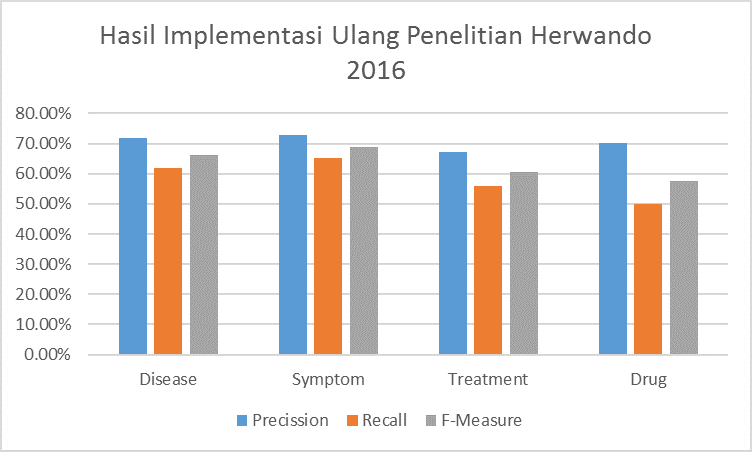
\includegraphics[width=0.85\linewidth]{images/radit}
	\caption{Histogram Metrik Evaluasi dengan Fitur Kata Itu Sendiri}
	\label{fig:radit}
\end{figure}

%-----------------------------------------------------------------------------%
\section{Skenario Eksperimen}
Pada penelitian ini, \saya~melakukan 2 buah skenario utama, yaitu skenario untuk menguji fitur yang memiliki kontribusi untuk meningkatkan akurasi dari setiap eksperimen dan skenario untuk menguji arsitektur RNNs yang \saya~usulkan. Berikut merupakan skenario yang \saya~rancang dalam penelitian ini:
\begin{enumerate}
	\item Skenario untuk menguji fitur\\
	Skenario ini bertujuan untuk mendapatkan kombinasi fitur terbaik sehingga memberikan akurasi terbaik. \Saya~mencoba masing-masing fitur dengan menggunakan model arsitektur LSTMs biasa. Apabila penggunaan fitur memberikan hasil yang lebih dari pada hasil eksperimen sebelumnya, fitur tersebut akan dipertahankan untuk eksperimen yang selanjutnya. Skenario ini memiliki 9 sub-skenario, yaitu:
	\begin{enumerate}
		\item Sub-skenario menguji fitur kata itu sendiri
		\item Sub-skenario menguji fitur terbaik sebelumnya ditambahkan fitur kamus
		\item Sub-skenario menguji fitur terbaik sebelumnya ditambahkan fitur stop word
		\item Sub-skenario menguji fitur terbaik sebelumnya ditambahkan fitur POS-Tag
		\item Sub-skenario menguji fitur terbaik sebelumnya ditambahkan fitur frasa kata
		\item Sub-skenario menguji fitur terbaik sebelumnya dikurangi fitur POS-Tag
		\item Sub-skenario menguji fitur terbaik sebelumnya ditambahkan fitur 1 kata sebelum
		\item Sub-skenario menguji fitur terbaik sebelumnya ditambahkan fitur 1 kata sesudah
	\end{enumerate}
	\item Skenario untuk menguji arsitektur RNNs\\
	Skenario ini bertujuan untuk melihat pengaruh arsitektur RNNs pada penelitian ini. \Saya~mencoba kedua arsitektur RNNs yang telah diusulkan sebelumnya dengan menggunakan kombinasi fitur terbaik dari eksperimen di skenario pengujian fitur di atas. Pada skenario ini, terdapat 2 sub-skenario, yaitu:
	\begin{enumerate}
		\item Sub-skenario untuk menguji arsitektur LSTMs 1 tingkat
		\item Sub-skenario untuk menguji arsitektur LSTMs layer bertingkat
	\end{enumerate}
	
\end{enumerate}

\section{Hasil Eksperimen dan Analisis}
%-----------------------------------------------------------------------------%
Pada bagian ini akan dilaporkan hasil dari ekperimen yang telah \saya~rancang sesuai dengan skenario sebelumnya beserta analisisnya. 
	%-----------------------------------------------------------------------------%
	\subsection{Hasil Ekperimen Pengujian Fitur Beserta Analisis}
	
	Hasil eksperimen ini adalah laporan dari pengujian kombinasi fitur kata itu sendiri, kamus, \textit{stop word}, POS-Tag, frasa kata (frasa kata benda dan kata kerja), 1 kata sebelum, dan 1 kata sesudah.
	  
	\subsubsection{Sub-Eksperimen Menguji Fitur Kata itu Sendiri}
	%-----------------------------------------------------------------------------%
	Merujuk pada penelitian \cite{mujiono2016new}, penelitian tersebut bertujuan untuk mendapatkan \textit{non-handcrafted feature}, yaitu fitur kata itu sendiri dengan menggunakan \textit{tools Word Embedding}. Oleh karena itu, \saya~menguji fitur ini untuk mengetahui pengaruhnya pada program \mer~di penelitian ini. Tabel \ref{table:own1} menampilkan hasil pelabelan otomatis dengan menggunakan fitur kata itu sendiri yang direpresentasikan dengan menggunakan vektor \textit{word embedding}.
	
	\begin{table}
	    \centering
	    \caption{Tabel Hasil Eksperimen dengan Fitur Kata Itu Sendiri}
	    \begin{tabular}{|c|c|c|c|c|}
	      \hline
						      & \textit{Precision} & \f{\f{Recall}} & \f{\f{F-Measure}} \\ \hline
	      \textit{Disease}    & 61.38\%             & 60.42\%        & 60.37\%           \\ \hline
	      \textit{Symptom}    & 57.05\%             & 56.13\%        & 56.19\%           \\ \hline
	      \textit{Treatment}  & 49.92\%             & 47.17\%        & 46.96\%           \\ \hline
	      \textit{Drug}		  & 62.86\%             & 53.32\%        & 57.28\%           \\ \hline
	    \end{tabular}
	    \label{table:own1}
	\end{table}
	
	Pada tabel tersebut, dengan menggunakan fitur kata itu sendiri terlihat bahwa entitas \textit{Disease} memiliki \textit{recall} dan \textit{f-measure} tertinggi, yaitu 60.42\%, dan 60.37\%. Sedangkan entitas \textit{drug} memiliki \textit{precision} tertinggi, yaitu 62.86\%. Grafik \ref{fig:own1} menunjukkan perbandingan \textit{precision}, \textit{recall} dan \textit{f-measure} untuk masing-masing entitas.
	
	\begin{figure}
	  \centering
	  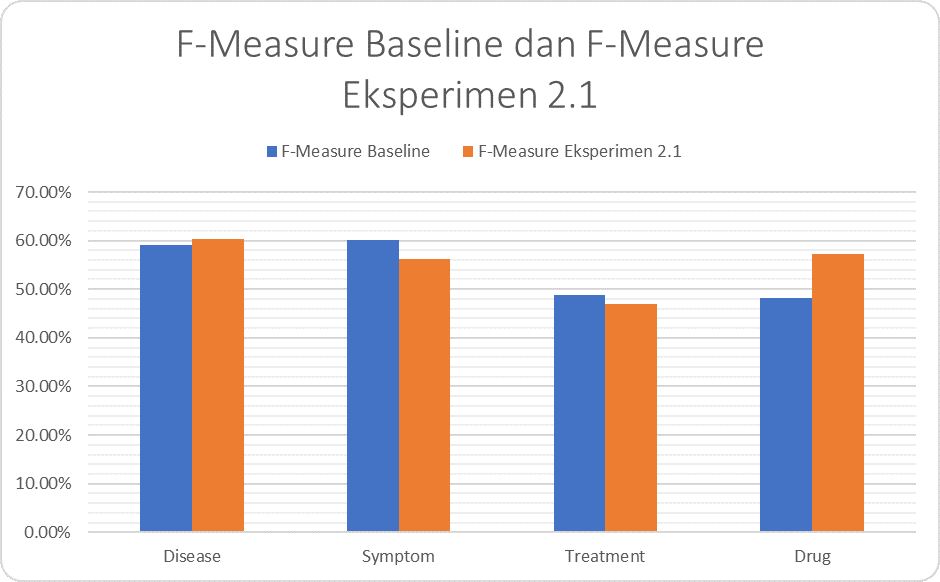
\includegraphics[width=0.85\linewidth]{images/histogram00}
	  \caption{Histogram Metrik Evaluasi dengan Fitur Kata Itu Sendiri}
	  \label{fig:own1}
	\end{figure}

	Pada eksperimen ini, ada beberapa nilai \textit{precision, recall} dan \textit{f-measure}  yang dicapai masih lebih kecil apabila dibandingkan dengan hasil yang dicapai \cite{skripsiKakRadit}. Menurut \saya~hal ini terjadi karena pada eksperimen ini hanya menggunakan fitur kata itu sendiri tanpa melibatkan informasi lain seperti pada penelitian yang dilakukan oleh \cite{skripsiKakRadit}. Oleh karena itu perlu adanya informasi lain, misalnya seperti apakah suatu kata terdapat dalam sebuah kamus kesehatan, informasi POS-Tag atau informasi yang lain. Oleh karena itu, \saya~mencoba menggunakan tambahan fitur lain untuk meningkatkan akurasi pada penelitian ini, yaitu pada sub-eksperimen \ref{eks:subeksdict}.
	
	%-----------------------------------------------------------------------------%
	\subsubsection{Sub-Eksperimen Menguji Fitur Terbaik Sebelumnya Ditambahkan Fitur Kamus Kesehatan (\textit{Disease, Symptom, Treatment} dan \textit{Drug})}\label{eks:subeksdict}
	%-----------------------------------------------------------------------------%
	Pada sub-eksperimen ini, \saya~menggunakan tambahan fitur Kamus Kesehatan karena berdasarkan penelitian \cite{skripsiKakRadit} fitur ini memiliki konribusi untuk menambah akurasi pada sistem \mer. Selain itu, menurut \saya, informasi suatu kata terdapat dalam sebuah kamus kesehatan mungkin akan memberikan kontribusi untuk meningkatkan akurasi. Oleh karena itu, \saya~mencoba untuk menambahkan fitur ini ke dalam model RNNs.
	
	Tabel \ref{table:owndict2} merupkan tabel hasil eksperimen yang didapatkan dengan menggunakan fitur ini.
	
	\begin{table}
		\centering
		\caption{Tabel Hasil Eksperimen dengan Fitur Terbaik Sebelumnya Ditambahkan Fitur Kamus Kesehatan}
		\begin{tabular}{|c|c|c|c|c|}
			\hline
			                      & \textit{Precision} & \f{\f{Recall}} & \f{\f{F-Measure}} \\ \hline
			\textit{Disease}      & 67.32\%             & 61.78\%        & 64.10\%           \\ \hline
			\textit{Symptom}      & 60.55\%             & 55.12\%        & 57.41\%           \\ \hline
			\textit{Treatment}    & 52.21\%             & 44.18\%        & 47.02\%           \\ \hline
			\textit{Drug}		  & 59.42\%             & 59.71\%        & 57.90\%           \\ \hline
		\end{tabular}
		\label{table:owndict2}
	\end{table}
	
	Berikut merupakan grafik yang merepresentasikan Tabel \ref{table:owndict2} dalam bentuk histogram.
	
	\begin{figure}
		\centering
		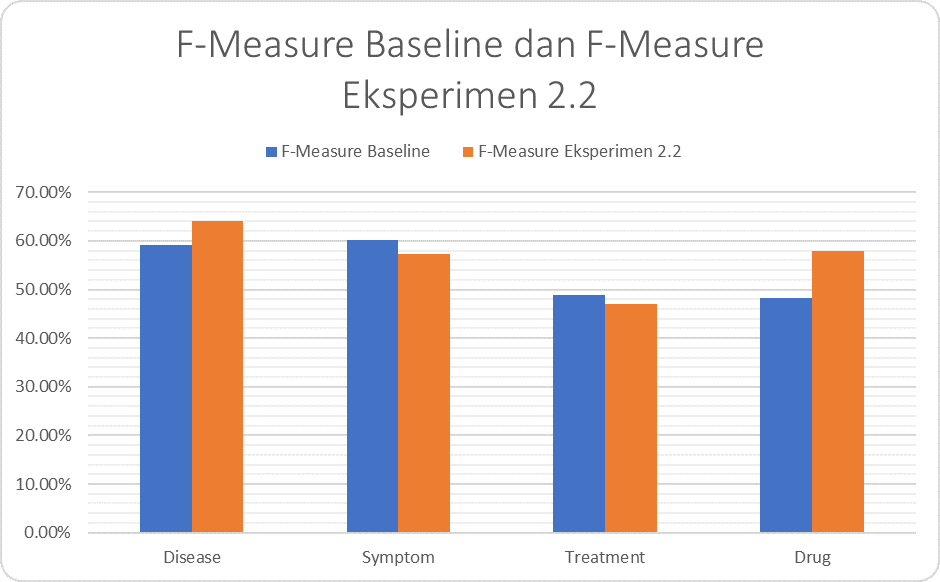
\includegraphics[width=0.85\linewidth]{images/histogram2}
		\caption{Histogram Metrik Evaluasi dengan Fitur Terbaik Sebelumnya Ditambahkan Fitur Kamus Kesehatan}
		\label{fig:owndict2}
	\end{figure}

	Dari tabel dan grafik tersebut, didapatkan informasi bahwa dengan menggunakan tambahan fitur kamus kesehatan terlihat bahwa entitas \textit{Disease} mengalami kenaikan nilai \textit{precision}, \textit{recall}, dan \textit{f-measure}. Selain itu, entitas \textit{symptom} dan \textit{tratment} mengalami kenaikan nilai \textit{precision} dan \textit{f-measure}. Entitas \textit{drug} mengalami penurunan pada nilai \textit{precision} namun mengalami kenaikan pada nilai \textit{recall} dan \textit{f-measure}-nya. Secara keseluruhan,  Sedangkan entitas \textit{drug} memiliki \textit{precission} tertinggi, yaitu 62.86\%. Grafik \ref{fig:owndict2} menunjukkan perbandingan \textit{precision}, \textit{recall} dan \textit{f-measure} untuk masing-masing entitas.
	
	Dari analisis yang \saya~lakukan terhadap korpus dan kamus kesehatan, terdapat beberapa entitas pada korpus yang tidak terdapat pada kamus sehingga mengakibatkan kenaikan hasil tidak banyak. Hal ini karena terdapat beberapa penyebab, yaitu:
	\begin{enumerate}
		\item Ada entitas yang merupakan kombinasi atau gabungan dari entitas lain yang dihubungkan dengan kata penghubung. Hal ini banyak \saya~temukan pada entitas \textit{treatment} dan \textit{symptom}. Contoh dari kasus ini yaitu:
		\begin{itemize}
			\item nyeri hebat dibagian ulu hati dan pinggang belakang (gabungan dari "nyeri hebat dibagian ulu hati" dan "nyeri hebat pinggang belakang")
			\item kondisi fases berampas , kuning , sedikit berlendir (gabungan dari "kondisi fases berampas", "kondisi fases kuning" dan "kondisi fases sedikit berlendir")
			\item alis atas dan bibir tidak bisa digerakkan (gabungan dari "alis atas tidak bisa digerakkan" dan "bibir tidak bisa digerakkan")
		\end{itemize}
		
		\item Penggunaan kata ganti orang di dalam entitas. Contoh dari kasus ini yaitu:
		\begin{itemize}
			\item suara \textbf{saya} hilang
			\item gusi \textbf{saya} berdarah
			\item pinggang \textbf{saya} sakit
		\end{itemize}
		
		\item Kesalahan eja pada entitas atau penggunaan kata yang tidak baku, misalnya:
		\begin{itemize}
			\item radang paru 2
			\item butawarna
			\item jrawatan
			\item kanker darah setadium 1
		\end{itemize}
	\end{enumerate}

	Dibandingkan dengan hasil eksperimen \cite{skripsiKakRadit}, hasil yang dicapai pada eksperimen ini masih lebih rendah pada entitas \textit{symptom} dan \textit{treatment}. Menurut \saya~perlu ada informasi tambahan untuk meningkatkan akurasi. Seperti yang kita ketahui bahwa eksperimen \cite{skripsiKakRadit} tidak hanya menggunakan fitur kata itu sendiri dan kamus kesehatan saja. Oleh karena itu, \saya~mencoba melakukan eksperimen kembali dengan menggunakan tambahan fitur lain pada sub-eksperimen \ref{eks:subekstopword};
	
	%-----------------------------------------------------------------------------%
	\subsubsection{Sub-Eksperimen Menguji Fitur Terbaik Sebelumnya Ditambahkan Fitur Stopword}\label{eks:subekstopword}
	%-----------------------------------------------------------------------------%
	Pada sub-eksperimen ini. \saya~mencoba menambahkan informasi lain berupa fitur yang berisi sebuah kata apakah terdapat di dalam kamus \textit{stop word} atau tidak. \Saya~berpendapat bahwa dengan adanya informasi \textit{stop word}, adanya kesalahan suatu kata tidak berentitas yang dilabeli sebagai kata berentitas oleh model dapat dikurangi.
	
	Rangkuman hasil sub-eksperimen ini dapat dilihat di Tabel \ref{table:owndict3} dan Gambar \ref{fig:owndict3}.
	
	\begin{table}
		\centering
		\caption{Tabel Hasil Eksperimen dengan Fitur Terbaik Sebelumnya Ditambahkan Fitur Stopword}
		\begin{tabular}{|c|c|c|c|c|}
			\hline
							      & \textit{Precision} & \f{\f{Recall}} & \f{\f{F-Measure}} \\ \hline
			\textit{Disease}      & 65.97\%             & 59.81\%        & 62.28\%           \\ \hline
			\textit{Symptom}      & 63.08\%             & 55.20\%        & 58.68\%           \\ \hline
			\textit{Treatment}    & 54.73\%             & 46.27\%        & 49.69\%           \\ \hline
			\textit{Drug}		  & 61.88\%             & 58.99\%        & 59.57\%           \\ \hline
		\end{tabular}
		\label{table:owndict3}
	\end{table}
		
	\begin{figure}
		\centering
		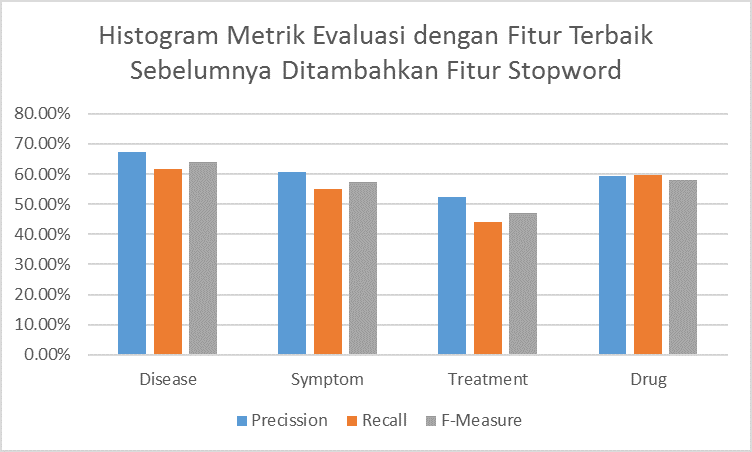
\includegraphics[width=0.85\linewidth]{images/histogram3}
		\caption{Histogram Metrik Evaluasi dengan Fitur Terbaik Sebelumnya Ditambahkan Fitur Stopword}
		\label{fig:owndict3}
	\end{figure}
	
	Dari Tabel \ref{table:owndict3} dan Gambar \ref{fig:owndict3} dapat diamati bahwa secara umum, penggunaan fitur kamus \textit{stop word} dapat meningkatkan \textit{precision, recall,} dan \textit{f-measure}. Untuk lebih detailnya, entitas \textit{disease} mengalami penurunan nilai \textit{precision} dan \textit{f-measure} tetapi mengalami kenaikan nilai \textit{recall}. Entitas \textit{symptom} dan \textit{treatment} mengalami kenaikan untuk nilai \textit{precision, recall} dan \textit{f-measure}. Sedangkan entitas \textit{drug} mengalami kenaikan pada nilai \textit{precission} dan \textit{f-measure} teteapi mengalami penurunan pada nilai \textit{recall}.
		
	Pada sub-eksperimen ini, walaupun secara umum akurasi lebih baik dibandingkan dengan sub-eksperimen sebelumnya, hasil sub-eksperimen ini masih lebih rendah pada entitas \textit{treatment} apabila dibandingkan dengan hasil eksperimen \cite{skripsiKakRadit}. Oleh karena \saya~mengusulkan fitur tambahan lain yaitu fitur POS-Tag yang akan dijelaskan pada sub-eksperimen \ref{eks:subekspostag}.
	
	%-----------------------------------------------------------------------------%
	\subsubsection{Sub-Eksperimen Menguji Fitur Terbaik Sebelumnya Ditambahkan Fitur POS-Tag}\label{eks:subekspostag}
	%-----------------------------------------------------------------------------%
	Pada sub-eksperimen ini, \saya~menambahkan informasi baru pada \textit{resource} yang akan digunakan untuk \textit{training} model yang berupa fitur POS-Tag. Sebelumnya fitur ini telah digunakan pada penelitian \cite{abacha2011medical} pada dokumen berbahasa Inggris dan memberikan kontribusi meningkatkan akurasi dari model \mer~yang dibangun. Oleh karena itu pada eksperimen ini \saya~mencoba menggunakan fitur tersebut dan ingin mengetahui apakah fitur POS-Tag memiliki kontribusi untuk meningkatkan akurasi pada \mer~dengan dokumen berbahasa Indonesia. 
	
	Rangkuman hasil sub-eksperimen ini dapat dilihat pada Tabel \ref{table:owndict4} dan Gambar \ref{fig:owndict4}.
	
	\begin{table}
		\centering
		\caption{Tabel Hasil Eksperimen dengan Fitur Terbaik Sebelumnya Ditambahkan Fitur POS-Tag}
		\begin{tabular}{|c|c|c|c|c|}
			\hline
								  & \textit{Precision} & \f{\f{Recall}} & \f{\f{F-Measure}} \\ \hline
			\textit{Disease}      & 69.10\%             & 58.67\%        & 63.22\%           \\ \hline
			\textit{Symptom}      & 61.09\%             & 54.43\%        & 57.00\%           \\ \hline
			\textit{Treatment}    & 59.73\%             & 44.10\%        & 49.87\%           \\ \hline
			\textit{Drug}		  & 62.00\%             & 55.74\%        & 57.87\%           \\ \hline
		\end{tabular}
		\label{table:owndict4}
	\end{table}
	
	\begin{figure}
		\centering
		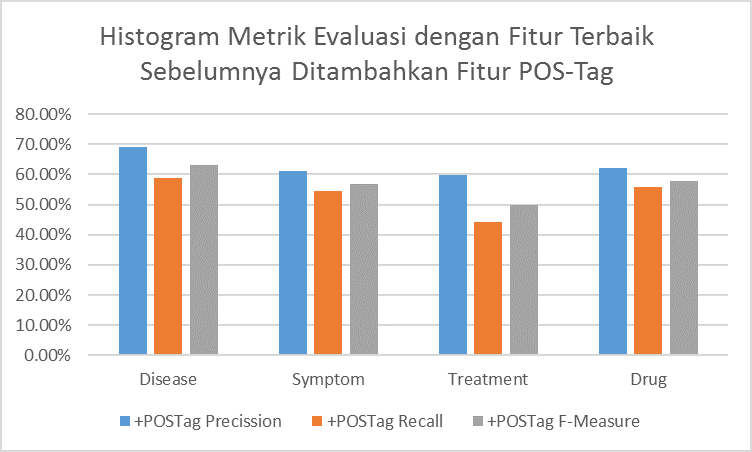
\includegraphics[width=0.85\linewidth]{images/histogram4}
		\caption{Histogram Metrik Evaluasi dengan Fitur Terbaik Sebelumnya Ditambahkan Fitur POS-Tag}
		\label{fig:owndict4}
	\end{figure}
	
	Dari tabel dan grafik di atas, entitas \textit{disease} dan \textit{treatment} memiliki nilai \textit{precision} dan \textit{f-measure} yang meningkat, tetapi dengan nilai \textit{recall} yang turun. Untuk entitas \textit{symptom}, nilai \textit{precision, recall}, dan \textit{f-measure} mengalami penurunan. Sedangkan entitas \textit{drug} mengalami kenaikan hanya pada \textit{precision}-nya saja.
	
	Hasil dari penggunaan fitur ini kurang baik, karena beberapa hal, yaitu:
	\begin{enumerate}
		\item Tag yang dihasilkan tidak konsisten. Pada beberapa entitas, terkadang suatu kata mendapatkan tag "A", namun di entitas yang lain untuk kata yang sama mendapatkan tag yang berbeda. Contoh dari kasus ini yaitu:
		\begin{itemize}
			\item "antibiotik" memiliki tag "vb", sedangkan pada entitas lain "antibiotik" memiliki tag "NN"
			\item "sakit kepala" memiliki beberapa tag pada entitas berbeda, yaitu "CD NN", "JJ NN", dan "NN NN"
			\item "nyeri" memiliki beberapa tag pada entitas berbeda, yaitu "NN", "VB", "IN", "WH", dan "IN".
		\end{itemize}
		\item Tidak ada perbedaan tag antara kata berentitas dengan tidak, misalnya nama orang mendapatkan tag "NN" (intan\_NN lusia\_NN), namun nama penyakit juga mendapatkan tag "NN" (Kanker\_NN Otak\_NN).
		\item Model POS-Tagger yang digunakan merupakan model untuk kalimat dengan topik umum, tidak dikhususkan pada topik kesehatan.
	\end{enumerate}
	
	Oleh karena itu pada sub-eksperimen selanjutnya, \saya~mencoba menambahkan fitur lain yang lebih spesifik dibandingkan dengan fitur POS-Tag, yaitu fitur Frasa Kata. Penjelasan lebih lanjut akan dibahas pada sub-eksperimen \ref{eks:subeksfrasa}.
	
	%-----------------------------------------------------------------------------%
	\subsubsection{Sub-Eksperimen Menguji Fitur Terbaik Sebelumnya Ditambahkan Fitur Frasa Kata}\label{eks:subeksfrasa}
	%-----------------------------------------------------------------------------%
	Pada sub-eksperimen ini \saya~menambahkan fitur baru yaitu fitur Frasa Kata. Seperti yang telah dijelaskan pada Bab 3, entitas \textit{symptom} dan \textit{treatment} diharapkan akan lebih mudah dikenali karena pada umumnya merupakan frasa kata kerja. Sedangkan entitas \textit{disease} dan \textit{drug} diharapkan juga akan lebih mudah dikenali karena pada umumnya merupakan frasa kata benda.
	
	Rangkuman hasil sub-eksperimen ini dapat dilihat pada Tabel \ref{table:owndict4} dan Gambar \ref{fig:owndict4}.
	
	\begin{table}
		\centering
		\caption{Rangkuman Hasil Eksperimen dengan Fitur Terbaik Sebelumnya Ditambahkan Fitur Frasa Kata}
		\begin{tabular}{|c|c|c|c|c|}
			\hline
			                      & \textit{Precision} & \f{\f{Recall}} & \f{\f{F-Measure}} \\ \hline
			\textit{Disease}      & 67.49\%             & 61.56\%        & 63.81\%           \\ \hline
			\textit{Symptom}      & 62.89\%             & 52.27\%        & 56.72\%           \\ \hline
			\textit{Treatment}    & 54.87\%             & 44.92\%        & 49.06\%           \\ \hline
			\textit{Drug}		  & 59.77\%             & 53.37\%        & 55.66\%           \\ \hline
		\end{tabular}
		\label{table:owndict5}
	\end{table}

	\begin{figure}
		\centering
		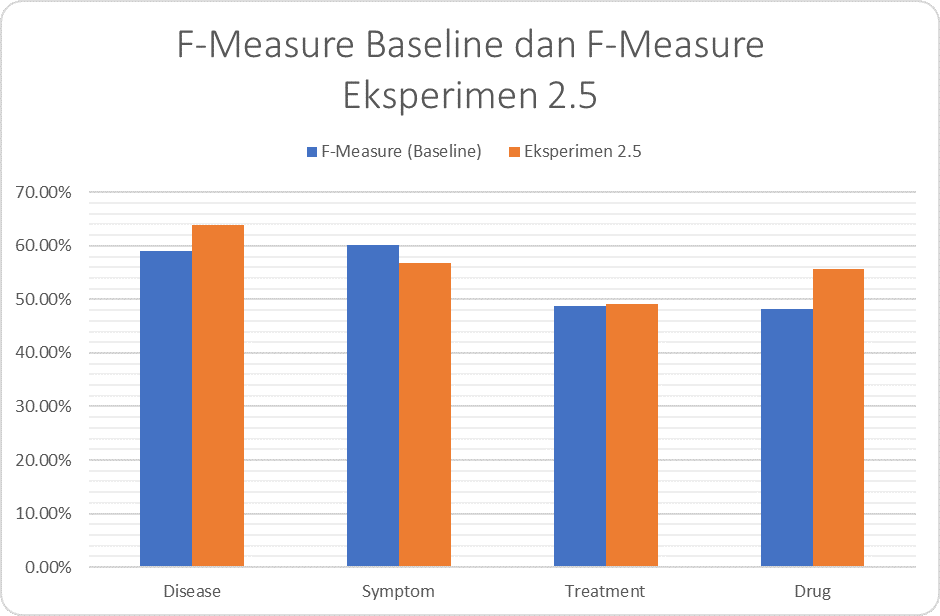
\includegraphics[width=0.85\linewidth]{images/histogram5}
		\caption{Histogram Metrik Evaluasi dengan Fitur Terbaik Sebelumnya Ditambahkan Fitur Frasa Kata}
		\label{fig:owndict5}
	\end{figure}

	Dari tabel dan grafik di atas, entitas \textit{drug} mengalami penurunan untuk nilai \textit{precission, recall} dan \textit{f-measure}. Selain itu, entitas \textit{disease} mengalami penurunan pada nilai \textit{precission} tetapi mengalami kenaikan pada nilai \textit{recall} dan \textit{f-measure}. Entitas \textit{symptom} mengalami kenaikan pada nilai \textit{precision} tetapi mengalami penurunan pada nilai \textit{recall} dan \textit{f-measure}. Sedangkan pada entitas \textit{treatment}, terjadi kenaikan nilai \textit{recall} tetapi nilai \textit{precision} dan \textit{f-measure} mengalami penurunan. 
	
	Dari korpus yang \saya~miliki, berikut merupakan informasi statistik dari penggunaan fitur frasa kata kerja:
	\begin{enumerate}
		\item Untuk entitas \textit{disease}, sebanyak 442 entitas merupakan frasa kata benda, 31 entitas merupakan bagian dari frasa kata benda dan 583 entitas bukan merupakan frasa.
		\item Untuk entitas \textit{symptom}, sebanyak 486 entitas merupakan frasa kata benda, 194 entitas merupakan bagian dari frasa kata benda dan 626 entitas bukan merupakan frasa.
		\item Untuk entitas \textit{treatment}, sebanyak 338 entitas merupakan frasa kata benda, 76 entitas merupakan bagian dari frasa kata benda dan 401 entitas bukan merupakan frasa.
		\item Untuk entitas \textit{drug}, sebanyak 152 entitas merupakan frasa kata benda, 8 entitas merupakan bagian dari frasa kata benda dan 194 entitas bukan merupakan frasa.
	\end{enumerate}
	
	
	Dari korpus yang \saya~miliki, berikut merupakan informasi statistik dari penggunaan fitur frasa kata benda:
	\begin{enumerate}
		\item Untuk entitas \textit{disease}, sebanyak 943 entitas merupakan frasa kata benda, 43 entitas merupakan bagian dari frasa kata benda dan 70 entitas bukan merupakan frasa.
		\item Untuk entitas \textit{symptom}, sebanyak 842 entitas merupakan frasa kata benda, 363 entitas merupakan bagian dari frasa kata benda dan 101 entitas bukan merupakan frasa.
		\item Untuk entitas \textit{treatment}, sebanyak 561 entitas merupakan frasa kata benda, 201 entitas merupakan bagian dari frasa kata benda dan 53 entitas bukan merupakan frasa.
		\item Untuk entitas \textit{drug}, sebanyak 318 entitas merupakan frasa kata benda, 14 entitas merupakan bagian dari frasa kata benda dan 22  entitas bukan merupakan frasa.
	\end{enumerate}
	Dari informasi di atas, dapat diambil informasi bahwa sebagian besar entitas \textit{disease} dan \textit{drug} merupakan frasa kata benda. Hal ini menjadi seharusnya menjadi informasi pembeda dengan kata lain. Namun apabila dilihat dari hasil eksperimen ini, performa penggunaan fitur ini tidak terlalu bagus atau bahkan turun di kedua entitas tersebut. \Saya~berpendapat hal ini terjadi karena penggunaan fitur ini redundan dengan penggunaan fitur POS-Tag.
	
	Dari hasil eksperimen ini, menurut \saya~hal ini terjadi karena informasi frasa bersifat redundan apabila bergabung dengan fitur POS-Tag. Pada fitur POS-Tag, tidak ada perbedaan antara kata yang merupakan frasa maupun kata yang bukan frasa. Padahal, mayoritas entitas merupakan frasa. Oleh karena itu, pada sub-eksperimen \ref{eks:subeksminpostag}, penulis menghilangkan fitur POS-Tag dan tetap mempertahankan fitur frasa Kata untuk mengetahui hal tersebut. 
	
	%-----------------------------------------------------------------------------%
	\subsubsection{Sub-Eksperimen Menguji Fitur Terbaik Sebelumnya Dikurangi Fitur POS-Tag}\label{eks:subeksminpostag}
	%-----------------------------------------------------------------------------%
	Pada sub-eksperimen ini \saya~menghilangkan fitur POS-Tag berdasarkan hasil dan analisis pada sub-eksperimen \ref{eks:subeksfrasa}. Rangkuman hasil sub-eksperimen ini dapat dilihat pada Tabel \ref{table:owndict6} dan Gambar \ref{fig:owndict6}.
	
	\begin{table}
		\centering
		\caption{Rangkuman Hasil Eksperimen dengan Fitur Terbaik Sebelumnya Dikurangi Fitur POS-Tag}
		\begin{tabular}{|c|c|c|c|c|}
			\hline
			                      & \textit{Precision} & \f{\f{Recall}} & \f{\f{F-Measure}} \\ \hline
			\textit{Disease}      & 68.67\%             & 61.80\%        & 64.78\%           \\ \hline
			\textit{Symptom}      & 63.79\%             & 56.10\%        & 59.23\%           \\ \hline
			\textit{Treatment}    & 54.47\%             & 46.72\%        & 49.58\%           \\ \hline
			\textit{Drug}		  & 60.08\%             & 56.70\%        & 57.00\%           \\ \hline
		\end{tabular}
		\label{table:owndict6}
	\end{table}
	
	\begin{figure}
		\centering
		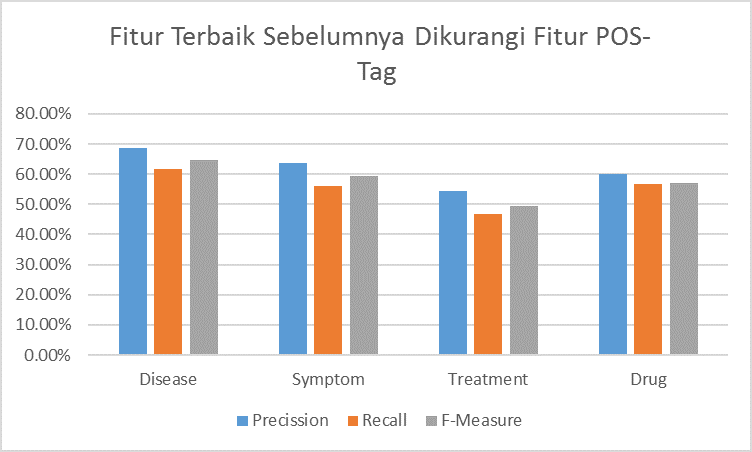
\includegraphics[width=0.85\linewidth]{images/histogram6}
		\caption{Histogram Metrik Evaluasi dengan Fitur Terbaik Sebelumnya Dikurangi Fitur POS-Tag}
		\label{fig:owndict6}
	\end{figure}
	
	Dari Tabel \ref{table:owndict6} dan Gambar \ref{fig:owndict6}, terlihat bahwa semua entitas (\textit{disease, symptom, treatment,}) dan \textit{drug} mengalami kenaikan pada nilai \textit{precision, recall,} dan \textit{f-measure}. Seperti yang telah dijelaskan pada sub-eksperimen \ref{eks:subeksfrasa}, penggabungan fitur POS-Tag dan frasa akan memberikan hasil yang lebih rendah. Oleh karena itu, sebaiknya fitur POS-Tag tidak digabung dengan fitur frasa. Selain itu, \saya~lebih memilih fitur frasa untuk dipertahankan karena fitur ini lebih diskriminatif dibandingkan dengan fitur POS-Tag, dengan melihat bahwa mayoritas kata berentitas merupakan frasa.
	
	Walaupun pada sub-eksperimen ini hasil yang dicapai lebih baik dari sub-eksperimen sebelumnya, hasilnya tetap lebih rendah dari hasil eksperimen \cite{skripsiKakRadit} pada nilai \textit{recall} dan \textit{f-measure} entitas \textit{symptom}. Oleh karena itu \saya~mencoba fitur yang lain, yaitu fitur Kata Sebelum. Untuk penjelasan lebih lanjut akan dibahas pada sub-eksperimen \ref{eks:subekswbef1}.
	
	%-----------------------------------------------------------------------------%
	\subsubsection{Sub-Eksperimen Menguji Fitur Terbaik Sebelumnya Ditambahkan Fitur 1 Kata Sebelum}\label{eks:subekswbef1}
	%-----------------------------------------------------------------------------%
	Pada sub-eksperimen ini \saya~menambahkan fitur baru yaitu fitur 1 Kata Sebelum. Fitur ini digunakan pada penelitian \cite{skripsiKakRadit} yang juga berkontribusi memberikan hasil terbaik pada penelitiannya. Menurut \saya, ada beberapa entitas yang akan lebih mudah diketahui apabila diketahui kata sebelumnya. Misalnya kata "masuk angin", apabila hanya diberikan informasi kata "angin" tanpa kata "masuk", akan lebih sulit menentukan kata tersebut bagian dari suatu entitas \textit{disease} atau bukan. Oleh karena itu, pada sub-eksperimen ini saya mencoba menambahkan fitur tersebut.
	
	Rangkuman hasil sub-eksperimen ini dapat dilihat pada Tabel \ref{table:owndict7} dan Gambar \ref{fig:owndict7}.
	
	\begin{table}
		\centering
		\caption{Rangkuman Hasil Eksperimen dengan Fitur Terbaik Sebelumnya Ditambahkan Fitur 1 Kata Sebelum}
		\begin{tabular}{|c|c|c|c|c|}
			\hline
		                          & \textit{Precision} & \f{\f{Recall}} & \f{\f{F-Measure}} \\ \hline
			\textit{Disease}      & 69.49\%             & 61.60\%        & 64.68\%           \\ \hline
			\textit{Symptom}      & 64.78\%             & 57.15\%        & 60.23\%           \\ \hline
			\textit{Treatment}    & 56.58\%             & 44.71\%        & 49.54\%           \\ \hline
			\textit{Drug}		  & 62.22\%             & 57.28\%        & 58.76\%           \\ \hline
		\end{tabular}
		\label{table:owndict7}
	\end{table}
	
	\begin{figure}
		\centering
		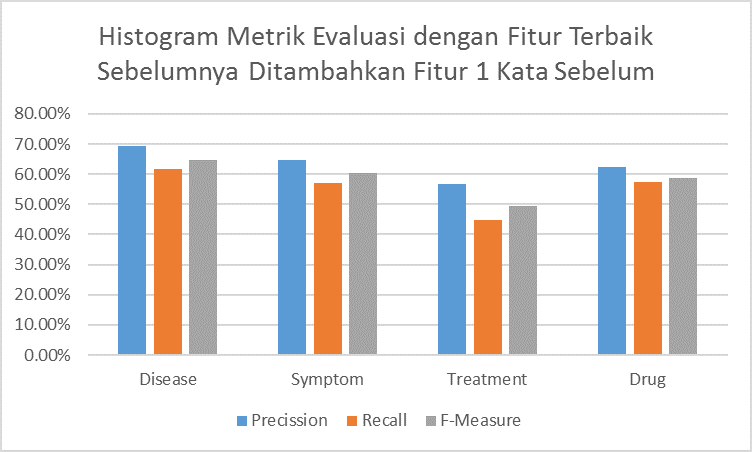
\includegraphics[width=0.85\linewidth]{images/histogram7}
		\caption{Histogram Metrik Evaluasi dengan Fitur Terbaik Sebelumnya Ditambahkan Fitur 1 Kata Sebelum}
		\label{fig:owndict7}
	\end{figure}
	
	Melihat pada Tabel \ref{table:owndict7} dan Gambar \ref{fig:owndict7}, dapat diketahui bahwa entitas \textit{disease} dan \textit{treatment} mengalami kenaikan pada nilai \textit{precission}, tetapi mengalami penurunan pada nilai \textit{recall} dan \textit{f-measure}. Sedangkan entitas \textit{symptom} dan \textit{drug} mengalami kenaikan pada nilai \textit{precision, recall,} dan \textit{f-measure}.
	
	Hasil sub-eksperimen ini masih lebih rendah dibandingkan dengan hasil eksperimen \cite{skripsiKakRadit} pada \textit{recall} dan \textit{f-measure} entitas \textit{treatment}. Oleh karena itu, \saya~mencoba menambahkan fitur yang lain yaitu fitur 1 Kata sesudah, yang akan dibahas lebih lanjut pada sub-eksperimen \ref{eks:subekswaf1}.
	
	
	%-----------------------------------------------------------------------------%
	\subsubsection{Sub-Eksperimen Menguji Fitur Terbaik Sebelumnya Ditambahkan Fitur 1 Kata Sesudah}\label{eks:subekswaf1}
	%-----------------------------------------------------------------------------%
	Pada sub-eksperimen ini \saya~menambahkan fitur lain yaitu fitur 1 Kata Setelah. Hal ini karena ada beberapa kasus yang mana apabila suatu kata merupakan sebuah entitas, akan lebih mudah dikenali apabila melihat kata atau konteks setelahnya. Sama seperti contoh pada fitur 1 kata sebelum, misal diberikan kata "masuk angin", apabila hanya diberikan informasi "masuk" tanpa "angin", akan lebih sulit mengenali apakah kata tersebut termasuk entitas \textit{disease} atau bukan. Selain itu, fitur ini juga dapat membedakan kata berentitas dengan kata yang bukan, misalnya kata "masuk angin" dengan "masuk rumah". Apabila informasi pada saat tersebut hanya diberikan kata "masuk" saja tanpa kata setelahnya, akan lebih sulit mengenali kata tersebut termasuk kata berentitas atau bukan.
	
	Rangkuman hasil sub-eksperimen ini dapat dilihat pada Tabel \ref{table:owndict8} dan Gambar \ref{fig:owndict8}.
	
	\begin{table}
		\centering
		\caption{Rangkuman Hasil Eksperimen dengan Fitur Terbaik Sebelumnya Ditambahkan Fitur 1 Kata Sesudah}
		\begin{tabular}{|c|c|c|c|c|}
			\hline
			& \textit{Precision} & \f{\f{Recall}} & \f{\f{F-Measure}} \\ \hline
			\textit{Disease}      & 70.68\%             & 66.18\%        & 68.17\%           \\ \hline
			\textit{Symptom}      & 64.16\%             & 59.55\%        & 61.42\%           \\ \hline
			\textit{Treatment}    & 61.02\%             & 51.13\%        & 54.03\%           \\ \hline
			\textit{Drug}		  & 70.85\%             & 70.33\%        & 69.82\%           \\ \hline
		\end{tabular}
		\label{table:owndict8}
	\end{table}
	
	\begin{figure}
		\centering
		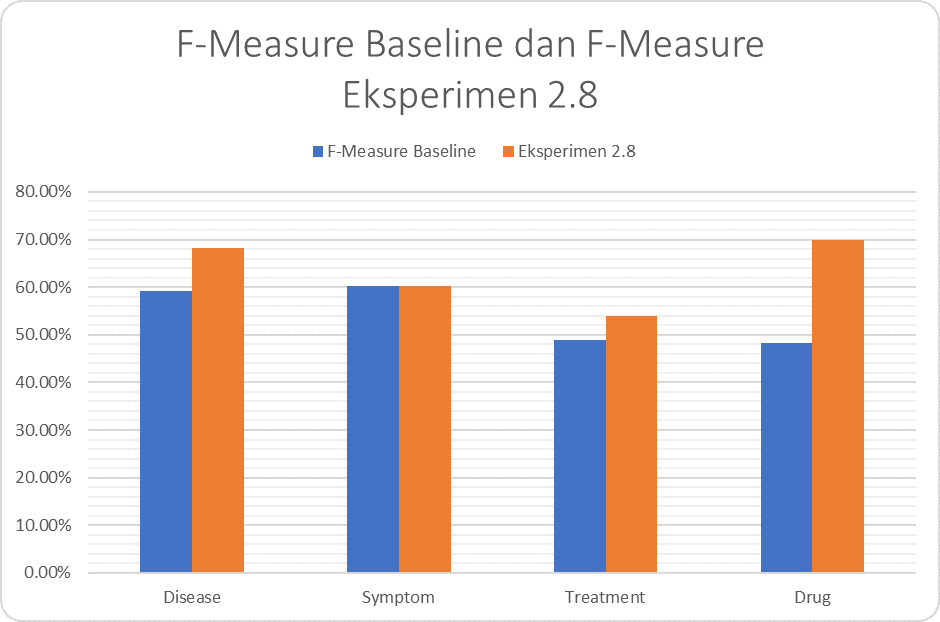
\includegraphics[width=0.85\linewidth]{images/histogram8}
		\caption{Histogram Metrik Evaluasi dengan Fitur Terbaik Sebelumnya Ditambahkan Fitur 1 Kata Sesudah}
		\label{fig:owndict8}
	\end{figure}
	
	Melihat pada Tabel \ref{table:owndict8} dan Gambar \ref{fig:owndict8}, dapat diketahui bahwa hanya entitas \textit{symptom} yang mengalami penurunan nilai pada \textit{precision}, tetapi nilai \textit{recall} dan \textit{f-measure}-nya naik. Sedangkan entitas lain mengalami kenaikan pada nilai \textit{precision, recall} dan \textit{f-measure}. Oleh karena itu, setelah \saya~mencoba kemungkinan fitur yang memberikan kontribusi dalam penelitian ini, \saya~mencoba arsitektur untuk model RNNs yang lain. Penjelasan lebih lanjut akan dibahas pada eksperimen \ref{eks:eks2}.
	
	
	
  %-----------------------------------------------------------------------------%
  
  
    \subsection{Hasil Ekperimen Pengujian Arsitektur RNNs}\label{eks:eks2}
    
    Pada eksperimen ini, \saya~mencoba dua buah arsitektur RNNs yang telah \saya~usulkan pada Bab 3 yaitu RNNs dengan 1 layer dan RNNs dengan 2 layer. Fitur yang digunakan dalam pengujian ini yaitu kombinasi fitur yang menghasilkan akurasi terbaik pada eksperimen pertama, yaitu fitur kata itu sendiri, kamus kesehatan, \textit{stop word}, frasa kata, 1 kata sebelum dan 1 kata sesudah.
    
    \subsubsection{Sub-Eksperimen Menguji Arsitektur LSTMs 1 tingkat}\label{eks2:subeksrnn1}
    %-----------------------------------------------------------------------------%
    Pada sub-eksperimen ini, \saya~menggunakan struktur RNNs yang mana semua fitur digabung menjadi satu dalam sebuah \textit{timestep}.
    Artinya fitur-fitur yang berbeda tersebut akan digabung atau di-\textit{concat} menjadi sebuah vektor yang akan menjadi \textit{input} bagi LSTMs ini. LSTMs inilah yang digunakan pada eksperimen pertama, sehingga hasilnya sama dengan sub-eksperimen \ref{eks:subekswaf1}.
    
    \begin{table}
    	\centering
    	\caption{Rangkuman Hasil Eksperimen dengan Arsitektur RNNs 1 Layer}
    	\begin{tabular}{|c|c|c|c|c|}
    		\hline
    		& \textit{Precision} & \f{\f{Recall}} & \f{\f{F-Measure}} \\ \hline
    		\textit{Disease}      & 70.68\%             & 66.18\%        & 68.17\%           \\ \hline
    		\textit{Symptom}      & 64.16\%             & 59.55\%        & 61.42\%           \\ \hline
    		\textit{Treatment}    & 61.02\%             & 51.13\%        & 54.03\%           \\ \hline
    		\textit{Drug}		  & 70.85\%             & 70.33\%        & 69.82\%           \\ \hline
    	\end{tabular}
    	\label{table:owndict9}
    \end{table}
    
    \begin{figure}
    	\centering
    	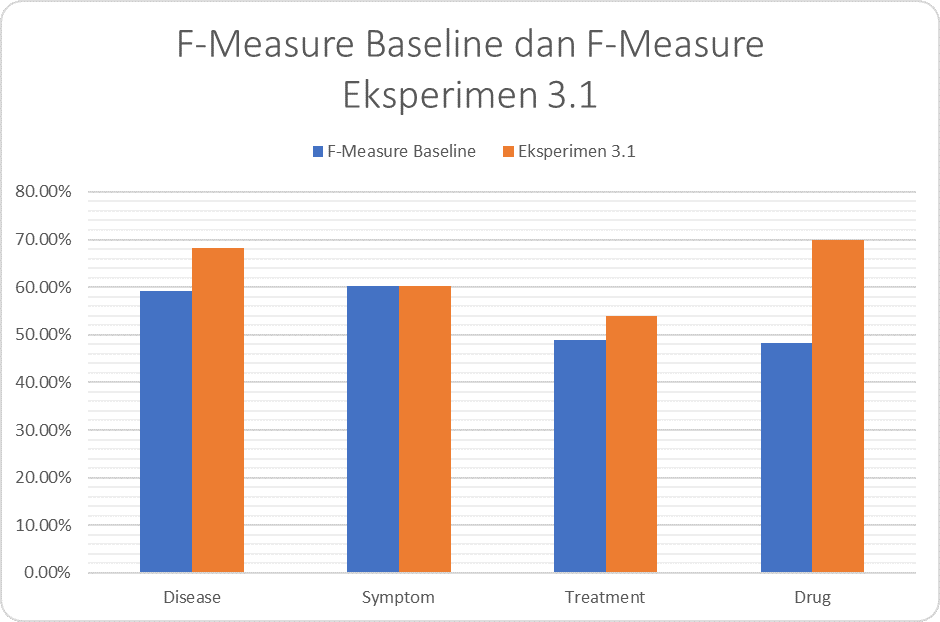
\includegraphics[width=0.85\linewidth]{images/histogram9}
    	\caption{Histogram Metrik Evaluasi dengan Arsitektur RNNs 1 Tingkat}
    	\label{fig:owndict9}
    \end{figure}
    
    Pada eksperimen ini, hasil yang sudah lebih baik apabila dibandingkan dengan hasil yang dicapai \cite{skripsiKakRadit} di entitas. Namun, dari eksperimen sebelumnya, terdapat akurasi yang turun, yaitu nilai \textit{precision} untuk entitas \textit{symptom}. Menurut \saya~hal ini terjadi karena informasi fitur yang berbeda-beda dijadikan satu, sehingga ada kemungkinan hilangnya informasi dari masing-masing fitur tersebut. Oleh karena itu, untuk mengatasi permasalahan tersebut \saya~mengusulkan arsitektur yang mana masing-masng kelompok fitur yang berbeda dipisahkan dan menjadi \textit{input} bagi masing-masing LSTMs. Untuk penjelasan eksperimen ini akan dijelaskan pada sub-eksperimen \ref{eks2:subeksrnn2}
    
    
    \subsubsection{Sub-Eksperimen Menguji Arsitektur LSTMs Layer Bertingkat}\label{eks2:subeksrnn2}
    %-----------------------------------------------------------------------------%
    Pada sub-eksperimen sebelumnya, fitur-fitur yang berbeda digabung menjadi satu, sehingga ada kemungkinan hilangnya informasi dari fitur tersebut. Oleh karena itu, \saya~mengusulkan adanya layer tambahan setelah masing-masing fitur tersebut masuk ke dalam model. \Saya~mengusulkan bahwa masing-masing kelompok fitur menjadi \textit{input} LSTMs secara terpisah. Setelah masuk di RNNs, \textit{output} dari masing-masing LSTMs tersebut di-\textit{merge} ke dalam sebuah layer, lalu masuk kembali ke LSTMs untuk melihat konteks fitur-fitur sebelumnya. Dengan diusulkannya arsitektur RNNs ini \saya~berharap bahwa masing-masing fitur terjaga informasinya dan tidak terganggu dengan informasi lain.
    
    Rangkuman hasil sub-eksperimen ini dapat dilihat pada Tabel \ref{table:owndict10} dan Gambar \ref{fig:owndict10}.
        
    \begin{table}
    	\centering
    	\caption{Rangkuman Hasil Eksperimen dengan Arsitektur RNNs 2 Layer}
    	\begin{tabular}{|c|c|c|c|c|}
    		\hline
    		& \textit{Precision} & \f{\f{Recall}} & \f{\f{F-Measure}} \\ \hline
    		\textit{Disease}      & 67.47\%             & 67.19\%        & 66.31\%           \\ \hline
    		\textit{Symptom}      & 64.90\%             & 60.63\%        & 62.13\%           \\ \hline
    		\textit{Treatment}    & 63.92\%             & 53.13\%        & 56.51\%           \\ \hline
    		\textit{Drug}		  & 66.39\%             & 62.33\%        & 63.61\%           \\ \hline
    	\end{tabular}
    	\label{table:owndict10}
    \end{table}
    
    \begin{figure}
    	\centering
    	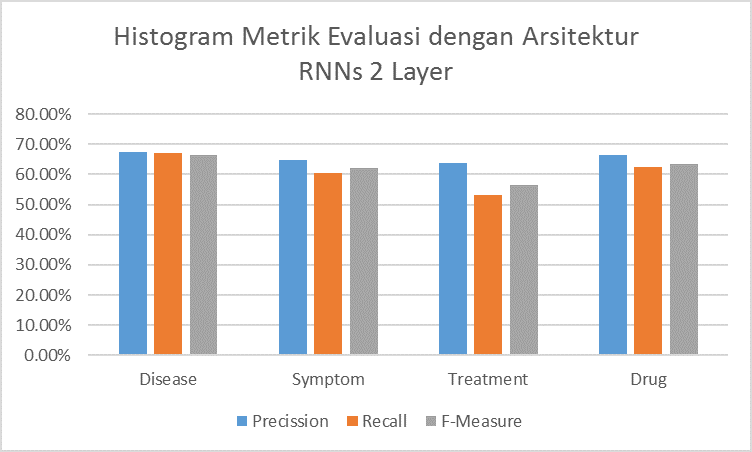
\includegraphics[width=0.85\linewidth]{images/histogramrnnv2}
    	\caption{Histogram Metrik Evaluasi dengan Arsitektur LSTMs Layer Bertingkat}
    	\label{fig:owndict10}
    \end{figure}

	Pada eksperimen ini, hasil yang sudah lebih baik apabila dibandingkan dengan hasil yang dicapai \cite{skripsiKakRadit} di masing-masing entitas dan lebih baik dibandingkan eksperimem \ref{eks2:subeksrnn1} pada identifikasi entitas \textit{symptom} dan \textit{treatment}.
